\subsection{Overview of 5G Network Architecture and A2G Communication}

The 5G mobile network is designed to support three main service objectives: Enhanced Mobile Broadband (eMBB) for high data rate services, Ultra-Reliable Low Latency Communications (URLLC) for delay-sensitive and reliable services, and Massive Machine-Type Communications (mMTC) for connecting a large number of devices \cite{itu_m2083}. In a basic 5G system, the UE is the terminal device that accesses the mobile network. A UE can be a smartphone, an Internet of Things (IoT) device, or in an aerial communication scenario, an unmanned aerial vehicle (UAV) acting as an aerial UE.

The UE connects to the radio access network (RAN) through a base station (BS), referred to in 5G as a gNB. The gNB is responsible for providing the wireless radio interface, transmitting and receiving radio signals, managing radio resources, and maintaining the radio connection with the UE. It also forwards user data and control information between the UE and the 5G Core (5GC) network. Therefore, the gNB is the main network element that directly determines how the UE accesses the 5G system over the air interface.

In a conventional terrestrial scenario, the UE is usually located near the ground and moves inside the coverage area of surrounding gNBs. The radio link quality is mainly affected by the horizontal distance between the UE and the serving gNB, obstacles such as buildings or terrain, shadow fading, and interference from neighboring cells.

Air-to-ground (A2G) communication extends this model by considering a UAV or aerial UE communicating with ground-based gNBs. This corresponds to the cellular-connected UAV case, where the UAV acts as a flying mobile terminal within a cellular network \cite{mozaffari2019tutorial,zeng2019accessing}. Unlike a ground UE, an aerial UE operates at a certain altitude and can have LOS or near-LOS paths to several BSs. This difference changes the radio propagation condition because the signal quality is affected not only by horizontal distance, but also by altitude, three-dimensional distance, and the elevation angle between the UAV and each gNB \cite{zeng2016uav}.

As the UAV moves, these geometric factors can change continuously. A higher altitude may improve visibility to the serving gNB, but it may also expose the UAV to stronger interference from multiple neighboring gNBs; this LoS-dominant channel and aerial-terrestrial interference are highlighted as key issues for UAV communications in 5G and beyond \cite{zeng2019accessing}. For this reason, important radio measurements such as RSRP and SINR may vary rapidly in A2G scenarios. These variations make A2G communication an important case for studying radio measurement behavior and mobility-related problems in 5G networks.

\begin{figure}[H]
\centering
\begin{tikzpicture}[scale=0.9, every node/.style={font=\small}]
    \draw[thick] (-1.2,0) -- (8.0,0);

    \coordinate (serving) at (1.0,1.15);
    \coordinate (ue) at (4.1,3.2);
    \coordinate (ueproj) at (4.1,0);
    \coordinate (intone) at (6.7,1.15);
    \coordinate (inttwo) at (-0.4,1.15);

    \foreach \x/\name in {1.0/Serving gNB,6.7/Neighbor gNB,-0.4/Neighbor gNB}{
        \draw[thick] (\x,0) -- (\x,1.05);
        \draw[thick] (\x-0.32,0) -- (\x,1.05) -- (\x+0.32,0);
        \draw[thick] (\x-0.45,1.15) -- (\x+0.45,1.15);
        \node[below] at (\x,0) {\name};
    }

    \draw[fill=gray!15, thick] (ue) circle (0.18);
    \node[above] at (ue) {Aerial UE};
    \draw[densely dotted] (ue) -- (ueproj);

    \draw[arrow] (serving) -- node[above, sloped] {serving link} (ue);
    \draw[arrow, dashed] (intone) -- node[above, sloped] {interference} (ue);
    \draw[arrow, dashed] (inttwo) -- (ue);

    \draw[<->] (1.0,-0.35) -- node[below] {\(d_{2D}\)} (4.1,-0.35);
    \draw[<->] (4.35,0) -- node[right] {\(h_{\mathrm{UE}}\)} (4.35,3.2);
    \draw[<->] (1.12,1.34) -- node[above, sloped] {\(d_{3D}\)} (3.95,3.18);
\end{tikzpicture}
\caption{A2G radio scenario with serving-gNB connection, neighboring-gNB interference, and geometry-dependent link measurements}
\label{fig:a2g-radio-scenario}
\end{figure}

\subsection{Cellular Network and Mobility Models}

The spatial arrangement of gNBs and the movement pattern of UEs are important factors in cellular network analysis. The network layout determines the relative positions of serving and neighboring gNBs, while the mobility model determines how the UE position changes over time. These two elements directly influence propagation distance, received signal strength, interference, and mobility-related events. This thesis considers a hexagonal cellular layout and the Manhattan mobility model as the theoretical basis for representing the network geometry and UE movement.

\subsubsection{Hexagonal Cellular Network Model}

The hexagonal cellular model is a conceptual approximation used to represent the radio coverage of a BS. In an ideal isotropic environment, equal received-power contours around a BS would be approximately circular. Actual cell boundaries, however, are irregular because they are shaped by terrain, buildings, antenna patterns, propagation loss, and interference. Therefore, a hexagonal cell should not be interpreted as the exact physical coverage boundary of a gNB, but as a simplified geometric abstraction for network planning and analysis \cite{rappaport2002}.

Circular cells cannot cover a large two-dimensional area without leaving gaps or creating overlaps. Regular hexagons, in contrast, tessellate the plane exactly and approximate circular coverage more closely than the other regular polygons that can tessellate the plane \cite{rappaport2002}. The hexagonal representation consequently provides both a simple approximation of radio coverage and a consistent structure for placing neighboring gNBs. Each cell has six immediate neighbors, which facilitates the analysis of inter-cell interference, cell association, and handover (HO) behavior.

\begin{figure}[H]
\centering
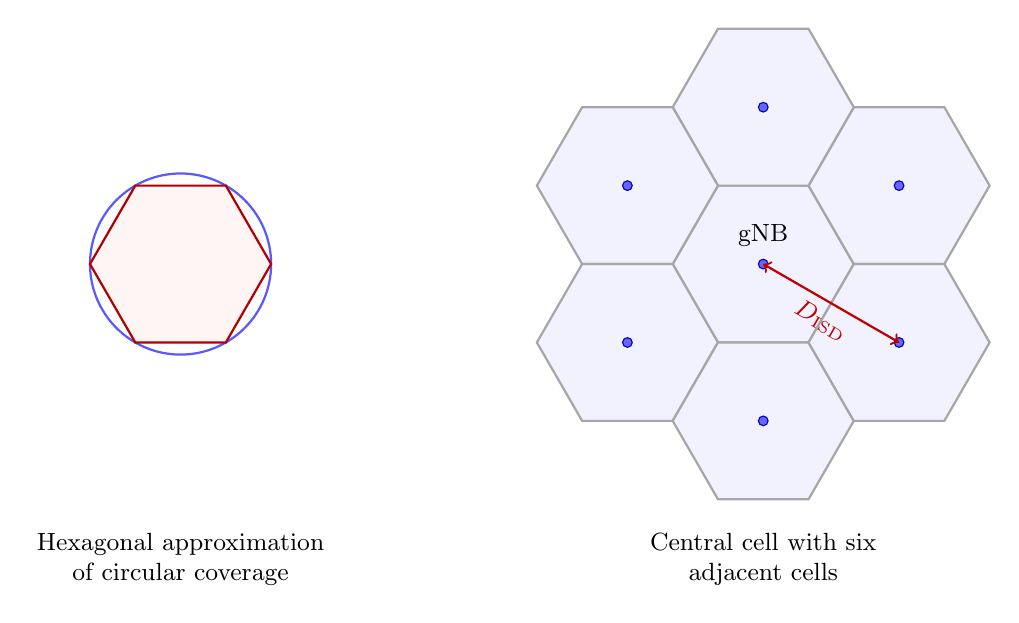
\begin{tikzpicture}[
    station/.style={
        circle,
        draw=blue!70!black,
        fill=blue!60,
        minimum size=3.5pt,
        inner sep=0pt
    }
]
\def\hexradius{1.15}

% Circular coverage approximation
\draw[blue!65, thick] (-3.8,0) circle[radius=\hexradius cm];
\draw[red!70!black, thick, fill=red!4]
    ({-3.8+\hexradius*cos(0)},   {\hexradius*sin(0)})
    \foreach \angle in {60,120,...,300} {
        -- ({-3.8+\hexradius*cos(\angle)}, {\hexradius*sin(\angle)})
    } -- cycle;
\node[align=center, font=\small] at (-3.8,-3.75)
    {Hexagonal approximation\\of circular coverage};

% Seven-cell hexagonal layout
\foreach \cx/\cy in {
    3.6/0,
    5.325/0.99593,
    3.6/1.99186,
    1.875/0.99593,
    1.875/-0.99593,
    3.6/-1.99186,
    5.325/-0.99593
}{
    \draw[gray!70, thick, fill=blue!5]
        ({\cx+\hexradius*cos(0)}, {\cy+\hexradius*sin(0)})
        \foreach \angle in {60,120,...,300} {
            -- ({\cx+\hexradius*cos(\angle)}, {\cy+\hexradius*sin(\angle)})
    } -- cycle;
    \node[station] at (\cx,\cy) {};
}
\draw[<->, thick, red!75!black] (3.6,0) -- node[below, sloped, font=\small] {$D_{\mathrm{ISD}}$} (5.325,-0.99593);
\node[above=3pt, font=\small] at (3.6,0) {gNB};
\node[align=center, font=\small] at (3.6,-3.75)
    {Central cell with six\\adjacent cells};
\end{tikzpicture}
\caption{Circular coverage approximation and seven-cell hexagonal layout}
\label{fig:hexagonal-cellular-layout}
\end{figure}

The distance between the centers of two adjacent cells is commonly referred to as the inter-site distance (ISD). For a regular hexagonal cell with radius \(R\), measured from the center to a vertex, the ISD is

\begin{equation}
    D_{\mathrm{ISD}} = \sqrt{3}R.
\end{equation}

The cell radius and ISD determine the spatial density of gNB deployment. A smaller ISD produces a denser network, which may improve coverage but also increases the possibility of inter-cell interference. Conversely, a larger ISD reduces the number of gNBs in a given area but may result in weaker received power near cell boundaries. Therefore, the hexagonal model is useful for studying coverage, neighboring-cell interference, cell association, and HO behavior.

\subsubsection{Manhattan Mobility Model}

The Manhattan mobility model is a geographic-restriction mobility model designed to represent movement on an urban street grid \cite{bai2003}. The service area is divided into horizontal and vertical road segments that form an orthogonal grid. A UE moves only along these road segments and may travel in one of four directions: North, South, East, or West. Direction changes are permitted at intersections, where the UE may continue forward or select another valid road while remaining inside the service area.

\begin{figure}[H]
\centering
\begin{tikzpicture}[
    road/.style={gray!65, line width=2.5pt},
    route/.style={-{Stealth[scale=0.9]}, red!75!black, line width=1.4pt},
    intersection/.style={circle, fill=black, minimum size=3pt, inner sep=0pt}
]
\foreach \x in {0,1.5,3,4.5,6}
    \draw[road] (\x,0) -- (\x,4.5);
\foreach \y in {0,1.5,3,4.5}
    \draw[road] (0,\y) -- (6,\y);
\foreach \x in {0,1.5,3,4.5,6}
    \foreach \y in {0,1.5,3,4.5}
        \node[intersection] at (\x,\y) {};
\draw[route] (0,1.5) -- (3,1.5) -- (3,3) -- (6,3);
\node[circle, draw=red!75!black, fill=red!15, minimum size=7mm] at (3,3) {\small UE};
\end{tikzpicture}
\caption{Example of UE movement in a Manhattan street grid}
\label{fig:manhattan-mobility}
\end{figure}

UE movement is considered continuous along each road segment. During one simulation interval, the travel distance is determined by the UE speed and the duration of the time step:

\begin{equation}
    d_{\mathrm{move}} = v \Delta t,
\end{equation}

where \(d_{\mathrm{move}}\) is the distance traveled during one time step, \(v\) is the UE speed, and \(\Delta t\) is the time-step duration. At an intersection, the movement direction may be updated according to the set of available directions. Additional behaviors such as temporary stops or gradual acceleration can also be included to represent traffic conditions, but they are not fundamental requirements of the Manhattan model.

The Manhattan model provides a more structured representation of urban mobility than unconstrained random movement. As the UE moves along the street grid, its distance and relative direction to surrounding gNBs change over time. These changes lead to variations in path loss, shadow fading, RSRP, and SINR, and may eventually cause the UE to change its serving gNB. Thus, the combination of the hexagonal network model and Manhattan mobility model provides a geometric foundation for studying radio measurements and HO behavior in a cellular network.

\subsection{Radio Propagation in 5G Networks and Measurement Metrics}

Radio propagation describes how the transmitted electromagnetic signal changes before it reaches the receiver. In a 5G cellular network, the received signal is affected by distance, carrier frequency, antenna gains, LOS or NLOS condition, shadowing objects, interference from other cells, and receiver noise. 3GPP TR 38.901 provides the commonly used channel-modelling framework for frequencies from 0.5 GHz to 100 GHz, including path loss, LOS probability, penetration loss, shadow fading, and fast-fading components for scenarios such as Urban Macro (UMa) and Urban Micro (UMi) \cite{3gpp_38901}. This thesis uses these concepts at a system-simulation level to generate interpretable radio measurements rather than to reproduce a full link-level channel realization.

For a UE and a gNB separated by horizontal distance \(d_{2D}\), the three-dimensional link distance is

\begin{equation}
    d_{3D} = \sqrt{d_{2D}^{2} + (h_{\mathrm{UE}} - h_{\mathrm{gNB}})^{2}},
\end{equation}

where \(h_{\mathrm{UE}}\) and \(h_{\mathrm{gNB}}\) are the UE and gNB antenna heights. This distance is especially important in A2G scenarios because a change in UE height changes both the link distance and the elevation geometry. A higher aerial UE may have a higher LOS probability to several gNBs, but the same visibility can also increase received interference from neighboring cells.

\subsubsection{Large-Scale Propagation Components Used in the Simulator}

The radio simulator uses a large-scale propagation abstraction rather than a full small-scale fading channel. This abstraction is appropriate for generating mobility traces because the quantities of interest are serving-cell strength, neighboring-cell strength, and SINR trends along the UE trajectory. The theoretical chain used in the simulator is

\begin{equation}
\{d_{2D},d_{3D},h_{\mathrm{UE}}\}
\rightarrow P_{\mathrm{LOS}}
\rightarrow S_{\mathrm{LOS/NLOS}}
\rightarrow PL
\rightarrow X_{\sigma}
\rightarrow \{P_{\mathrm{rx}},\mathrm{RSRP},\mathrm{SINR}\}.
\end{equation}

In this chain, geometry determines path length and LOS probability. The sampled LOS/NLOS state selects the path-loss formula. Shadow fading adds a spatially varying large-scale random term. Finally, the link budget and interference model convert these losses into received power, RSRP, and SINR.

\begin{table}[H]
\centering
\caption{Theoretical propagation components used by the radio simulator \cite{3gpp_38901,3gpp_36777,3gpp_38215}}
\small
\begin{tabularx}{\textwidth}{>{\raggedright\arraybackslash}p{3.0cm}>{\raggedright\arraybackslash}X>{\raggedright\arraybackslash}p{4.1cm}}
\toprule
Component & Theoretical role & Dataset quantity\\
\midrule
Link geometry & Defines horizontal distance, 3D distance, UE height, and the applicable terrestrial or aerial regime. & UE/gNB position, height, distance\\
LOS/NLOS condition & Represents the probability and realization of direct visibility between UE and gNB. & LOS probability, LOS state\\
Path loss & Models median large-scale attenuation due to distance, frequency, height, and propagation condition. & Path loss\\
Shadow fading & Models slow random variation around the median path loss caused by environmental obstruction. & Shadow-fading value\\
Link measurement & Converts propagation loss, antenna gains, noise, and interference into radio measurement indicators. & Received power, RSRP, SINR\\
\bottomrule
\end{tabularx}
\label{tab:theoretical-propagation-components}
\end{table}

\subsubsection{LOS Probability and LOS/NLOS State}

The simulator first calculates a LOS probability for each UE--gNB link. The model follows the UMa LOS probability in 3GPP TR 38.901 for terrestrial and low-height UEs and the UMa-AV extension in 3GPP TR 36.777 for aerial UEs \cite{3gpp_38901,3gpp_36777}. The NLOS probability is then

\begin{equation}
    P_{\mathrm{NLOS}} = 1 - P_{\mathrm{LOS}}.
\end{equation}

Here, \(\operatorname{clip}(x,0,1)\) denotes limiting \(x\) to the interval \([0,1]\). All distances in the following LOS-probability expressions are in metres.

The implemented LOS-probability calculation can be followed from the UE height range and then from the horizontal distance \(d_{2D}\). For terrestrial and low-height UEs, \(1.5 \le h_{\mathrm{UE}} \le 22.5\) m, the simulator uses the UMa expression from 3GPP TR 38.901 \cite{3gpp_38901}. If the UE is very close to the gNB in the horizontal plane, \(d_{2D}\le18\) m, the link is treated as LOS with

\begin{equation}
    P_{\mathrm{LOS}}=1.
\end{equation}

When \(d_{2D}>18\) m, the LOS probability decreases with distance but includes a height correction for UEs above 13 m:

\begin{align}
    P_{\mathrm{LOS}}
    &= \operatorname{clip}\left(P_{\mathrm{base}}G_h,0,1\right),\\
    P_{\mathrm{base}}
    &= \frac{18}{d_{2D}}+
       \left(1-\frac{18}{d_{2D}}\right)
       e^{-d_{2D}/63},\\
    G_h
    &= 1+\frac{5}{4}C(h_{\mathrm{UE}})
       \left(\frac{d_{2D}}{100}\right)^3
       e^{-d_{2D}/150}.
\end{align}

The height correction is inactive for ordinary ground-level UEs and becomes active only when \(h_{\mathrm{UE}}>13\) m:

\begin{equation}
C(h_{\mathrm{UE}})=
\begin{cases}
0, & h_{\mathrm{UE}}\le13,\\
\left(\dfrac{h_{\mathrm{UE}}-13}{10}\right)^{1.5},
& 13<h_{\mathrm{UE}}\le22.5.
\end{cases}
\end{equation}

For aerial UEs in the range \(22.5<h_{\mathrm{UE}}\le100\) m, the simulator switches to the UMa-AV LOS-probability model from 3GPP TR 36.777 \cite{3gpp_36777}. It first calculates two height-dependent parameters:

\begin{align}
    d_1 &= \max\left(460\log_{10}(h_{\mathrm{UE}})-700,18\right),\\
    p_1 &= 4300\log_{10}(h_{\mathrm{UE}})-3800.
\end{align}

The value \(d_1\) acts as the first horizontal-distance threshold. If \(d_{2D}\le d_1\), the link is treated as LOS:

\begin{equation}
    P_{\mathrm{LOS}}=1.
\end{equation}

If \(d_{2D}>d_1\), the LOS probability is reduced according to

\begin{equation}
    P_{\mathrm{LOS}}=
    \operatorname{clip}\left(
    \frac{d_1}{d_{2D}}+
    e^{-d_{2D}/p_1}
    \left(1-\frac{d_1}{d_{2D}}\right),
    0,1\right).
\end{equation}

Finally, for high aerial UEs, \(100<h_{\mathrm{UE}}\le300\) m, the implemented model sets

\begin{equation}
    P_{\mathrm{LOS}}=1.
\end{equation}

After \(P_{\mathrm{LOS}}\) is calculated, the simulator converts this probability into a concrete LOS/NLOS state by Bernoulli sampling. For each UE--gNB link, a uniform random variable \(u\sim\mathcal{U}(0,1)\) is drawn and the link state \(S\) is assigned as

\begin{equation}
S=
\begin{cases}
\mathrm{LOS}, & u \le P_{\mathrm{LOS}},\\
\mathrm{NLOS}, & u > P_{\mathrm{LOS}}.
\end{cases}
\end{equation}

Thus, a larger \(P_{\mathrm{LOS}}\) gives a higher chance that the link is realized as LOS, while \(P_{\mathrm{LOS}}=1\) always gives a LOS link and \(P_{\mathrm{LOS}}=0\) always gives a NLOS link. The sampled LOS/NLOS state is then cached once for each UE--gNB link and reused in the subsequent path-loss and shadow-fading calculations. This prevents the same link from randomly switching between LOS and NLOS at every time step and makes the generated trace easier to interpret.

\subsubsection{Path-Loss Model}

Path loss represents the large-scale attenuation between the transmitter and receiver. It increases with distance and depends on the propagation environment, carrier frequency, UE height, and LOS/NLOS state. The simulator follows the same order as the implementation in \texttt{radio\_models.py}: first it prepares effective distances, then it selects the UMa or UMa-AV formula according to UE height and sampled LOS/NLOS state. The low-height UMa formulas are based on 3GPP TR 38.901, and the aerial UMa-AV formulas are based on 3GPP TR 36.777 \cite{3gpp_38901,3gpp_36777}.

Before evaluating path loss, the horizontal distance is lower-bounded by 10 m and the effective 3D distance is recomputed:

\begin{align}
    d_{2D,\mathrm{eff}} &= \max(d_{2D},10),\\
    d_{3D,\mathrm{eff}} &=
    \sqrt{d_{2D,\mathrm{eff}}^2+
    (h_{\mathrm{gNB}}-h_{\mathrm{UE}})^2}.
\end{align}

For readability, the following path-loss equations use \(d_{2D}\) and \(d_{3D}\) to denote these effective distances after preprocessing.

The UMa LOS formula also uses the effective breakpoint distance

\begin{equation}
    d'_{\mathrm{BP}} =
    \frac{4(h_{\mathrm{gNB}}-1)(h_{\mathrm{UE}}-1)f_c}{c},
\end{equation}

where \(f_c\) is in Hz and \(c\) is the speed of light. In the remaining path-loss formulas, \(f_{c,\mathrm{GHz}}\) denotes the carrier frequency in GHz.

For \(1.5 \le h_{\mathrm{UE}} \le 22.5\) m, the simulator uses the UMa path-loss model. If the sampled link state is LOS and \(d_{2D}\le d'_{\mathrm{BP}}\), the LOS path loss is

\begin{equation}
    PL_{\mathrm{LOS}} =
    28+22\log_{10}(d_{3D})
    +20\log_{10}(f_{c,\mathrm{GHz}}).
\end{equation}

If the same low-height LOS link is beyond the breakpoint, \(d_{2D}>d'_{\mathrm{BP}}\), the slope changes to

\begin{align}
    PL_{\mathrm{LOS}} &=
    28+40\log_{10}(d_{3D})
    +20\log_{10}(f_{c,\mathrm{GHz}}) \nonumber\\
    &\quad -9\log_{10}\left(
    (d'_{\mathrm{BP}})^2+
    (h_{\mathrm{gNB}}-h_{\mathrm{UE}})^2
    \right).
\end{align}

If the sampled low-height link state is NLOS, the simulator first computes

\begin{align}
    PL'_{\mathrm{NLOS}} &=
    13.54+39.08\log_{10}(d_{3D})
    +20\log_{10}(f_{c,\mathrm{GHz}}) \nonumber\\
    &\quad -0.6(h_{\mathrm{UE}}-1.5),
\end{align}

and then applies the 3GPP max operation:

\begin{equation}
    PL_{\mathrm{NLOS}} =
    \max\left(PL_{\mathrm{LOS}},PL'_{\mathrm{NLOS}}\right).
\end{equation}

For aerial UEs, \(22.5<h_{\mathrm{UE}}\le300\) m, the LOS path-loss expression becomes the UMa-AV LOS formula:

\begin{equation}
    PL_{\mathrm{LOS,AV}} =
    28+22\log_{10}(d_{3D})
    +20\log_{10}(f_{c,\mathrm{GHz}}).
\end{equation}

For aerial NLOS links, the implemented UMa-AV NLOS expression is defined for \(22.5<h_{\mathrm{UE}}\le100\) m:

\begin{align}
    PL_{\mathrm{NLOS,AV}} &=
    -17.5+
    \left(46-7\log_{10}(h_{\mathrm{UE}})\right)
    \log_{10}(d_{3D}) \nonumber\\
    &\quad +20\log_{10}\left(
    \frac{40\pi f_{c,\mathrm{GHz}}}{3}
    \right).
\end{align}

The path loss stored in the dataset is selected according to the cached LOS/NLOS state:

\begin{equation}
PL =
\begin{cases}
PL_{\mathrm{LOS}}, & \text{for a low-height LOS link},\\
PL_{\mathrm{NLOS}}, & \text{for a low-height NLOS link},\\
PL_{\mathrm{LOS,AV}}, & \text{for an aerial LOS link},\\
PL_{\mathrm{NLOS,AV}}, & \text{for an aerial NLOS link with } 22.5<h_{\mathrm{UE}}\le100.
\end{cases}
\end{equation}

Thus, the logged path-loss value is not only a function of distance. It also reflects UE height, LOS probability, sampled LOS/NLOS state, carrier frequency, and the UMa or UMa-AV scenario selected for the link.

\subsubsection{Shadow-Fading Model}

Shadow fading models slower received-power variation caused by obstacles and local environmental structure that are not captured by distance-only path loss. It is commonly represented as a log-normal random component, or equivalently as a Gaussian random variable in dB. In the implemented simulator, the shadow-fading loss for a UE--gNB link is sampled as

\begin{equation}
    X_{\sigma}\sim\mathcal{N}(0,\sigma_{\mathrm{SF}}^2),
\end{equation}

where \(\sigma_{\mathrm{SF}}\) is selected from the corresponding LOS/NLOS and UE-height condition. For UMa-AV links, the standard deviation follows the shadow-fading parameters in 3GPP TR 36.777 Annex B, with the low-height UMa values referenced from TR 38.901 \cite{3gpp_36777,3gpp_38901}. The simulator uses

\begin{equation}
\sigma_{\mathrm{SF}} =
\begin{cases}
4~\mathrm{dB}, & 1.5\le h_{\mathrm{UE}}\le22.5~\mathrm{m},~\mathrm{LOS},\\
6~\mathrm{dB}, & 1.5\le h_{\mathrm{UE}}\le22.5~\mathrm{m},~\mathrm{NLOS},\\
4.64e^{-0.0066h_{\mathrm{UE}}}~\mathrm{dB}, & 22.5<h_{\mathrm{UE}}\le300~\mathrm{m},~\mathrm{LOS},\\
6~\mathrm{dB}, & 22.5<h_{\mathrm{UE}}\le100~\mathrm{m},~\mathrm{NLOS}.
\end{cases}
\end{equation}

For the default ground-UE mode, the implementation can also use fixed configured values, \(\sigma_{\mathrm{SF}}=4.6\) dB for LOS and \(10\) dB for NLOS, as defined in \texttt{config.py}. This separates the baseline terrestrial configuration from the UMa-AV height-dependent configuration used for aerial-UE studies.

The sampled value is clipped to the interval \([-3\sigma_{\mathrm{SF}},3\sigma_{\mathrm{SF}}]\). This clipping avoids unrealistically large random losses in finite simulation traces while preserving the zero-mean Gaussian behaviour for most samples. The received power including shadow fading is then

\begin{equation}
    P_{\mathrm{rx}} = P_{\mathrm{tx}} + G_{\mathrm{tx}} + G_{\mathrm{rx}} - PL - X_{\sigma},
\end{equation}

where \(P_{\mathrm{tx}}\) is the transmit power, \(G_{\mathrm{tx}}\) and \(G_{\mathrm{rx}}\) are antenna gains, \(PL\) is path loss, and \(X_{\sigma}\) is the shadow-fading term. A positive shadow-fading realization reduces the received power, while a negative realization improves it relative to the median path-loss value. This explains why two UE positions with similar distance to the serving gNB may still produce different received powers.

The simulator does not resample shadow fading independently at every time step. Instead, the current shadow-fading value is cached for each UE--gNB link and reused while the accumulated UE movement for that link remains below 25 m. Once the accumulated movement reaches 25 m, a new \(X_{\sigma}\) value is sampled and the accumulated distance is reset. This 25 m update distance implements a simple spatial-consistency approximation for large-scale fading, following the distance-dependent shadowing treatment used in 3GPP channel modelling \cite{3gpp_36777}. As a result, shadow fading changes more slowly than instantaneous RSRP or SINR calculations and avoids artificial step-to-step randomness in the generated measurement trace.

Reference Signal Received Power (RSRP) is a key measurement for assessing cell strength. In NR, 3GPP TS 38.215 defines SS-RSRP and CSI-RSRP as linear averages of the power contributions of resource elements carrying the corresponding synchronization-signal or CSI reference signals \cite{3gpp_38215}. In this thesis, RSRP is used as a system-level approximation of reference-signal power derived from the received downlink power. It provides a compact indicator of serving-cell and neighboring-cell strength and is therefore useful for comparing candidate gNBs along a UE trajectory.

Interference is produced by transmissions from non-serving cells that reuse the same time-frequency resources or overlap with the measured resources. Unlike thermal noise, interference depends on the topology, the UE position, the serving gNB, and the received powers from surrounding gNBs. A UE near a cell edge, or an aerial UE with LOS visibility to several gNBs, may observe strong desired-signal power and strong interference at the same time. For this reason, RSRP alone is not sufficient to describe link quality.

Receiver noise is commonly modelled from the thermal noise density and receiver noise figure:

\begin{equation}
    N_{\mathrm{dBm}} = -174 + 10\log_{10}(B) + NF,
\end{equation}

where \(B\) is the receiver bandwidth in Hz and \(NF\) is the receiver noise figure in dB. The value \(-174\) dBm/Hz is the approximate thermal noise power spectral density at room temperature \cite{rappaport2002}. Noise is independent of the serving-cell choice, but it becomes important when the received signal and interference powers are low.

Signal-to-Interference-plus-Noise Ratio (SINR) combines the desired signal, interference, and noise into one quality metric. In linear scale, it is written as

\begin{equation}
    \mathrm{SINR} = \frac{P_{\mathrm{serving}}}{\sum_{i=1}^{N_{\mathrm{int}}} P_{\mathrm{int},i} + P_{\mathrm{noise}}},
\end{equation}

and in dB as

\begin{equation}
    \mathrm{SINR}_{\mathrm{dB}} = 10\log_{10}(\mathrm{SINR}).
\end{equation}

3GPP TS 38.215 also specifies NR physical-layer SINR measurements, including SS-SINR and CSI-SINR, based on reference-signal resources and corresponding interference-plus-noise contributions \cite{3gpp_38215}. Conceptually, SINR is more directly related to link quality than RSRP because it penalizes both weak serving-signal power and strong interference. Thus, a UE can have acceptable RSRP but poor SINR if neighboring cells are received strongly.

The radio-measurement dataset generated in this thesis records these propagation and measurement concepts in structured form. UE position, height, velocity, and direction describe the mobility state. Serving-cell information identifies the current associated gNB. LOS probability and LOS state describe the propagation condition. Path loss, shadow fading, received power, RSRP, neighboring-cell RSRP, and SINR describe the radio environment observed by the UE at each simulation step. Together, these fields make it possible to inspect how movement changes radio conditions and how those changes may affect cell association and handover-related behavior.

\subsection{Handover in 5G Networks and Handover Delay}

???
định nghĩa. ví dụ: Handover delay is the time interval required for a UE to complete the transition from the source gNB to the target gNB.

\subsection{Chapter Conclusion}
This chapter presented the theoretical background related to 5G networks, A2G communication, radio propagation, radio measurement metrics, and handover delay. These concepts provide the foundation for the system design described in the next chapter.

